\documentclass[10pt]{article}
\usepackage[utf8]{inputenc}
\usepackage[a4paper, total={7in, 10in}]{geometry}
\usepackage{lipsum}
\usepackage{graphicx}
\usepackage{enumerate}
\usepackage{romannum}
\usepackage[table,xcdraw]{xcolor}
\renewcommand{\arraystretch}{1.2}
\usepackage{hyperref}
\hypersetup{hidelinks}
\hypersetup{
  colorlinks   = true, %Colours links instead of ugly boxes
  urlcolor     = red, %Colour for external hyperlinks
  linkcolor    = gray, %Colour of internal links
  citecolor   = red %Colour of citations
}
\usepackage{subfig}
\usepackage{placeins}




\title{\textbf{\fontsize{26}{12}\selectfont IEP Design Project – Sound to Light}}
\author{{\LARGE Lakee Sivaraya}\\[0.2in] CRSid : ls914\\[0.1in] Lab Group : 53}

\date{6 March 2021}


\newcommand{\img}[5]{

    \begin{figure}[h]
        \begin{center}
        \includegraphics[width=#1 \linewidth, height = #2\textheight, keepaspectratio]{#3} 
         \caption{#4}
        \label{fig:#5}      
        \end{center}
    
    \end{figure}

}

\newcommand{\bul}[1]{\begin{itemize}
    #1
\end{itemize}}

% title page
\begin{document}

\begin{titlepage}
\maketitle
    \centering
    \vfill
    {\bfseries\Large
     Emmanuel College\vspace{0.4in}
    }    
    
    
\includegraphics[width=3cm]{Emmanuel.pdf} 
    \vfill
    \vfill
    \thispagestyle{empty}

\end{titlepage}

\newpage
\section{Introduction}

The goal of the IEP Design Project was to design a \href{https://en.wikipedia.org/wiki/VU_meter}{VU meter} to visualize the amplitude of audio signals measured with a microphone. 
This lab report discuses the approach taken to design and build the device on a breadboard.

\section{Design}
    
    \begin{figure}[h]
        \begin{center}
        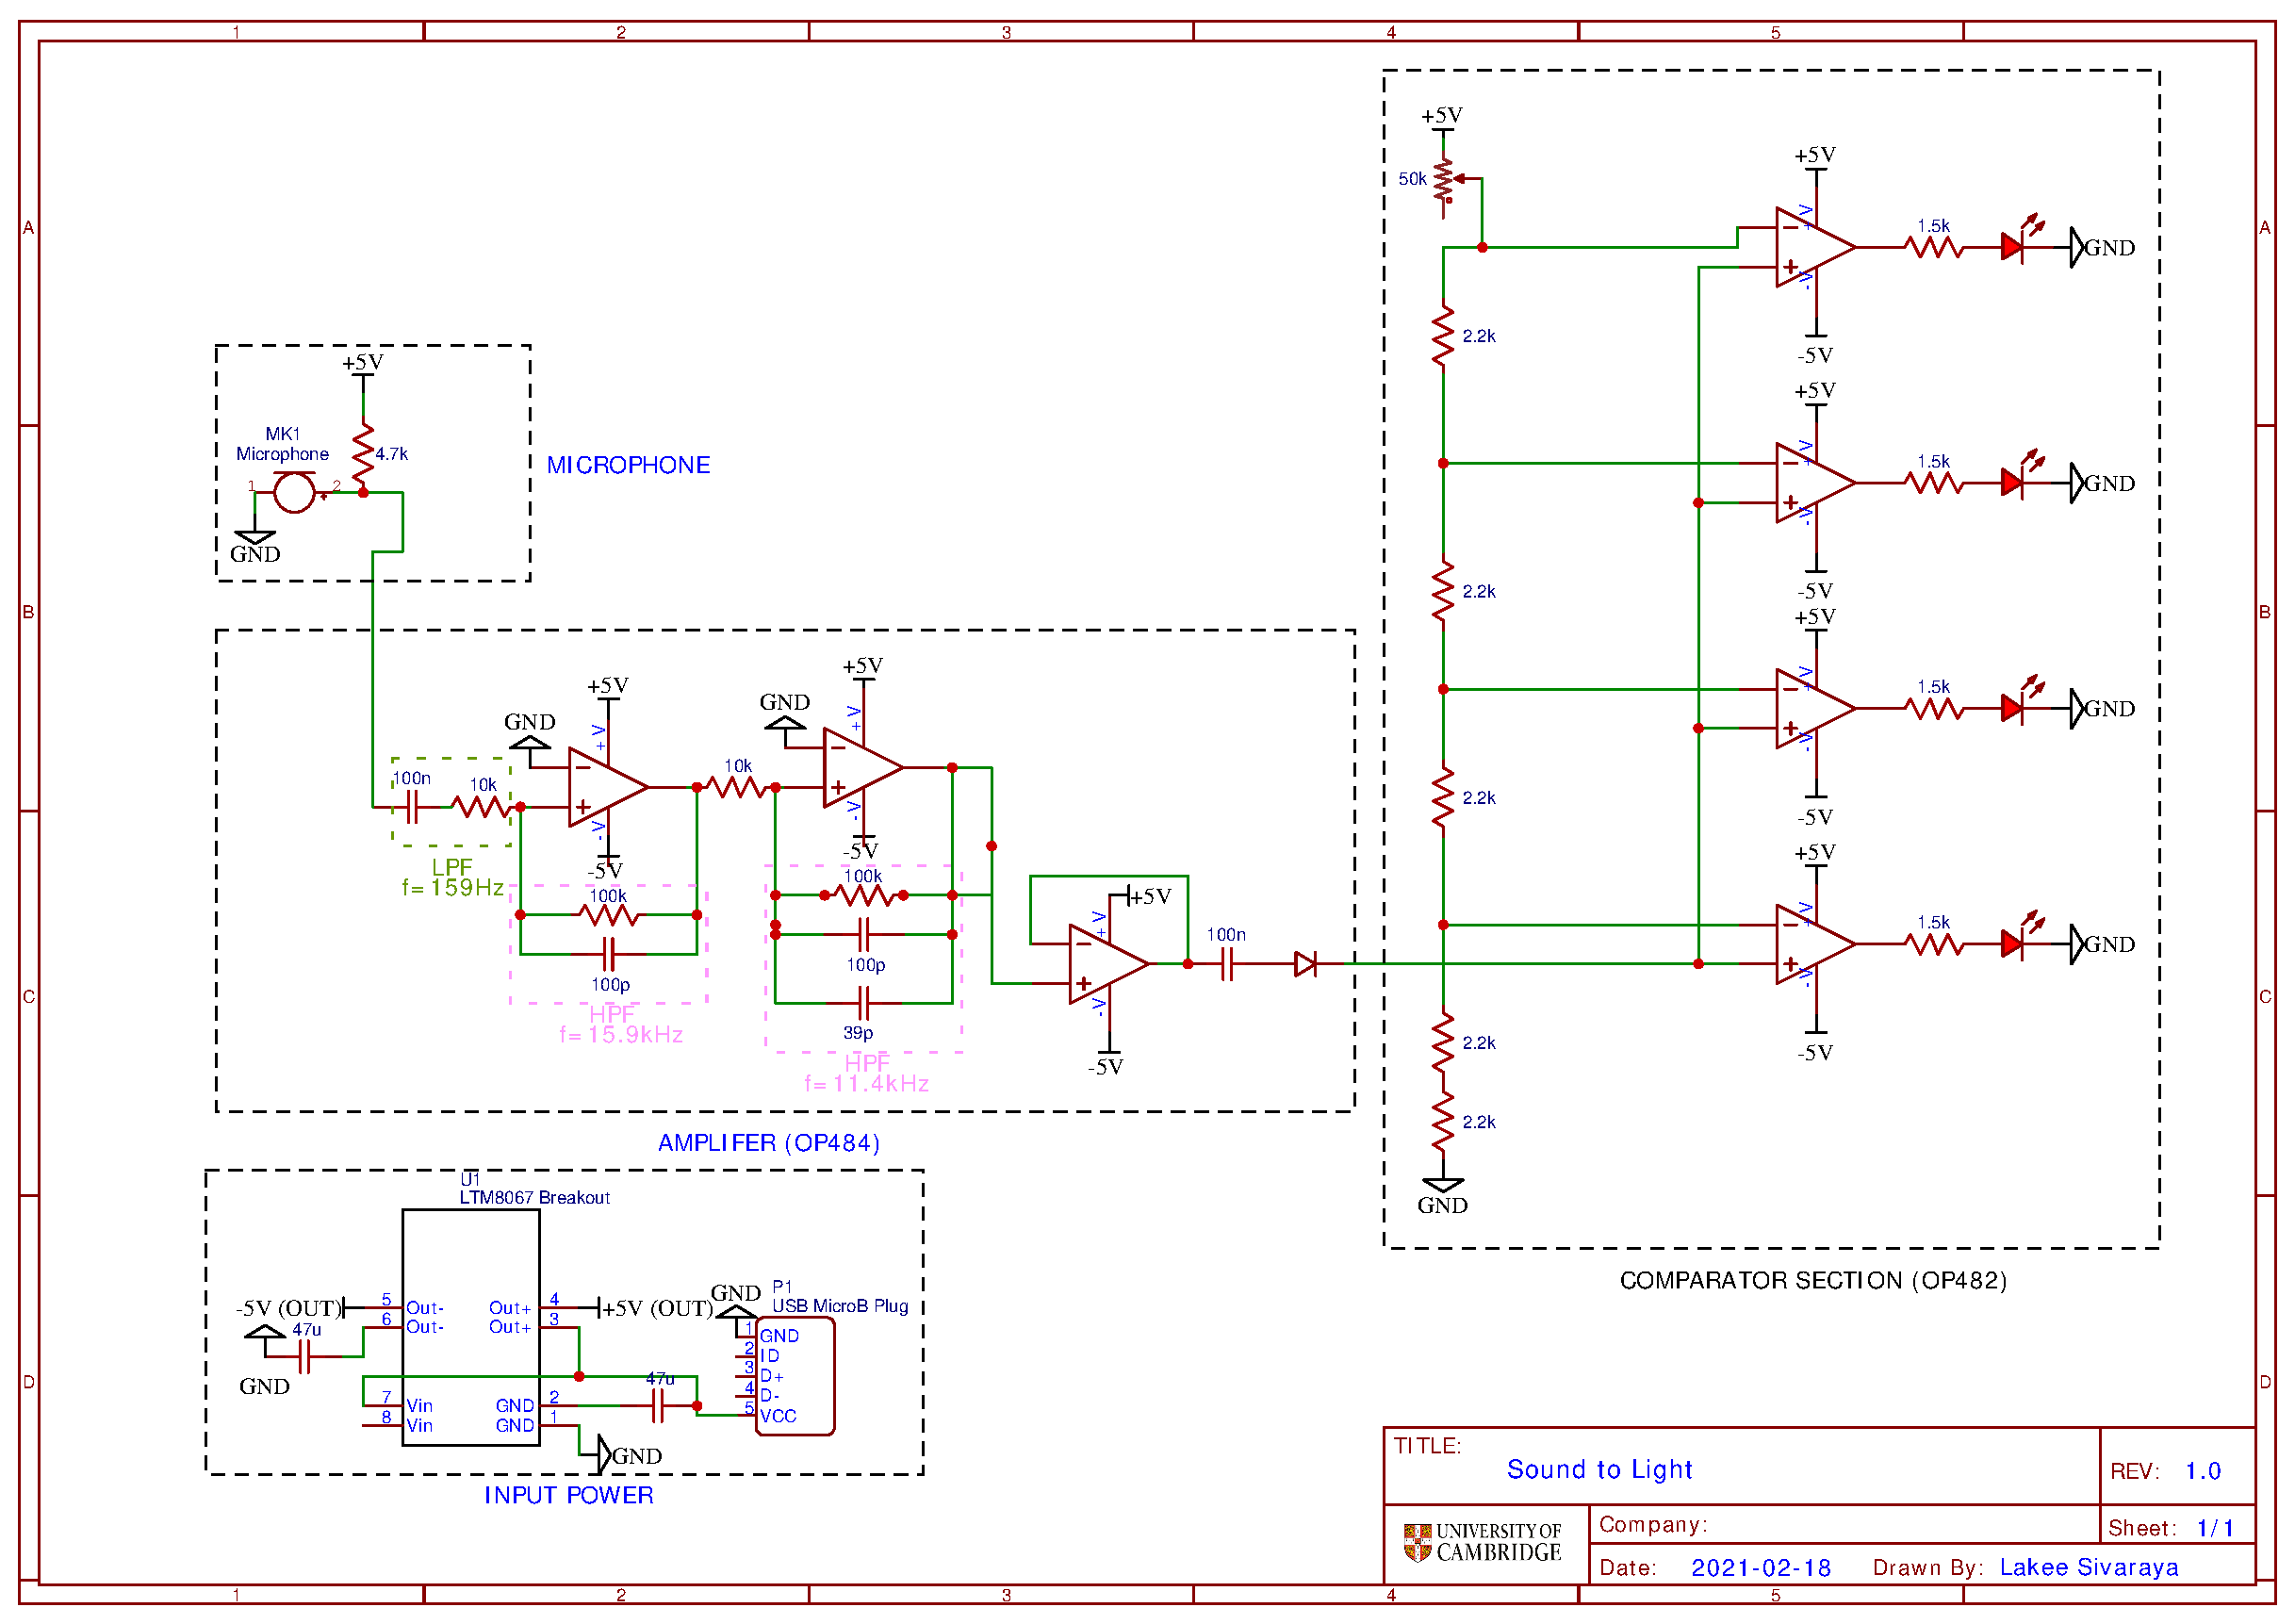
\includegraphics[width=\linewidth, height = 0.5\textheight, keepaspectratio]{schem.pdf} 
        \caption{Schematic of desgin split up into functional components}
        \label{fig:schem}      
        \end{center}
    \end{figure}
    
    \subsection{Input Power}
    The LTM8067 break out board was used to provide the $+5V$ and $-5V$ rails required to properly bias the OpAmps used in this circuit since they do not operate without a bipolar supply. $47\mu F$ capacitors were placed between the rails to reduce noise. 
    \subsection{Microphone}
    The microphone has an internal FET, so a $4.7k\Omega$ pull up resistor was connected between the ``drain" and $+5V$ rail to power the microphone and provide some amplification.
    \subsection{Amplifier}
    With a $1kHz$ sine test tone, it was found that the output of the microphone had an amplitude of $\sim5mV$. To get this voltage higher, the OP484 was used to chain two non-inverting amplifiers with individual gains of $\frac{100k\Omega}{10k\Omega}=10$ to  amplify the microphone signal by a factor $10^2=100$.
    
    \img{.9}{1}{filtered.png}{Output signal from a $1kHz$ test sound}{filtered}
    \noindent
    \vspace{-1.3em}
    \\Using a speaker to play a $1kHz$ test audio, the output from the amplifier, Figure \ref{fig:filtered}, showed that we got an amplification of around $565.7/5\approx 113$, which represent a small $13\%$ error from the theoretical gain.\\
    \noindent
    High and low pass filters (see Figure \ref{fig:schem}) were implemented with cutoffs of $f_{c,high}=159Hz$ and $f_{c,low}=15.9 , 11.4kHz$ respectively. These filters helped massively to filter out the noise (discussed in greater detail in \hyperref[sec:noise]{Section 3 - Noise}).
    \newline
     OpAmp buffer was connected after the OpAmp amplifiers to isolate the amplification section from the comparator section, thus preventing any unnecessary interference. After this buffer a $100nF$ capacitor were used to decouple the signal thus removing the small $0.1V$ DC offset present in the signal. Then the signal was rectified using a diode as we only need to consider the positive voltages in the comparator section.
    
    \subsection{Comparator}
    
    The comparator section used the 4 OpAmps on the OP482, to compare the input signal from the amplification (which was connected to the $V+$ pin), to a reference voltage (connected to the $V-$ pin). The output of each OpAmp is connected in series with an LED and a $1.5k\Omega$ current limiting resistor.
    When the signal goes above the reference, the output of the OpAmp goes to $+5V$ thus switches the LED on.\\
    A potential divider was used to create the voltage references. The divider uses a single $50k\Omega$ potentiometer in series with $2.2k\Omega$ resistors to create voltage references of $1.08,0.86,0.65,0.43V$ with the potentiometer was set at $\sim40k\Omega$. The reason why these voltage references were so high (much greater than $500mV$, see Figure \ref{fig:filtered}):
    \begin{enumerate}
    \item The voltage from real music (not the single frequency test tune) reached peaks of $1V$
    \item Noise (Figure \ref{fig:noise}) has an amplitude of around $0.2V$, meaning my lowest voltage reference should be higher than this
    \end{enumerate}

    \subsection{Breadboard Layout}
    \img{.7}{.8}{breadboard.jpg}{Breadboard Layout}{breadboard}
    \FloatBarrier
    \noindent
    One of the biggest challenge of this project was that we were only allowed to use components from the ADALP2000 kitset, meaning we were restricted to a small breadboard and the excessively long wires in the kitset.\\
    To circumvent this restriction, the metal ends of resistor were used to create connections between the holes, thus reducing the amount of jumper wires need and reduces clutter.
    

    
    


\section{Noise}
\label{sec:noise}
\img{.8}{1}{spectrum.png}{Spectrum analysis of noise}{spectrum}
\FloatBarrier
\noindent
Noise was easily the biggest issue that I faced during this project. From the spectrum in Figure \ref{fig:spectrum} we can see that there is a significant high frequency noise at around $130kHz$. The source of this noise is the transformer in the LTM8067 break out board. The strategies used to minimize the noise were:
\begin{enumerate}
    \item $47\mu F$ capacitors between the rails of the supply ``smoothing" out the noise.
    \item RC Low pass filters with cutoff frequencies well below the noise frequency to filter out the noise. Figure \ref{fig:lp} shows how powerful a simple RC low pass filer can be at removing the high frequencies from the noisy signal (red) and outputs a fairly clean signal (blue). The cut-off frequencies, $f_c$ of the filters were calculated using the equation,
    $$f_c=\frac{1}{2\pi RC}$$
    The chosen values of $f_c$ were $15.9kHz , 11.4kHz$, these values were chosen as they could be achieved using standard parts available in the kitset, and also most music does not have audio with frequencies higher than $10kHz$, which explains the fairly low values for the cutoff frequencies.
\end{enumerate}
\noindent
Additionally $50Hz$ noise was present in my signals due to the AC wires in the walls of my room. This noise is clearly evident in Figure \ref{fig:filtered} where you can see that there is some low frequency noise causing the sine waves to be slightly offset. To combat this, the signal from the microphone was filtered using an RC high pass filter with $f_c=159Hz$.


\img{.7}{1}{lp.PNG}{Filtering of the noise}{lp}
\FloatBarrier
\img{.7}{1}{noise.jpg}{Noise left after filtering (Timebase: $1s/div$)}{noise}
\FloatBarrier

\noindent
The strategies used to filter out the noise worked very well, however the noise did not completely disappear, leaving me with a $0.2V$ noise (Figure \ref{fig:noise}).\\ The main lesson learnt was that bipolar supplies should not be near the components that use it.
\section{Conclusion}
In conclusion, the designed VU meter clearly visualizes music (\href{https://drive.google.com/file/d/1vEgUyoO1fMyMp6ZBtADJIG7F9Pvy-P7P/view?usp=sharing}{video link}). The performance of my VU meter is the best that could be achieved with all the components that I have access to and the limited space for design. Noise caused many issues initially, but the strategies mentioned in \hyperref[sec:noise]{Section 3 - Noise} minimized its impact on the performance of my VU meter.

\end{document}




\end{document}
